\documentclass[../main.tex]{subfiles}
\begin{document}
%=========================================================
% TĐ_PBT_PRE1_HK1_Tuan14
% Phiếu bài tập PRE1 - Tuần 14
%   Toán: Làm quen với phép trừ, dấu trừ
%   Tiếng Việt: Làm quen âm d, đ
% Soạn theo mẫu (\hktuan, bt, listEX)
% Hình đặt trong thư mục Hinh_PRE1_Tuan14/ (cùng cấp với file này), tên hình có tiền tố p14_
% Đường dẫn tính từ thư mục của main.tex khi biên dịch main.tex
\graphicspath{{Hinh_PRE1_Tuan14/}{Data_PhieuBaiTap_HK0/Hinh_PRE1_Tuan14/}}
%=========================================================

%---------- Lệnh dùng chung cho phiếu ----------
% Chèn hình căn giữa, dính liền với đề bài phía trên (không bị tách trang)
% Tham số tùy chọn = chiều cao tối đa của hình (mặc định 8cm); hình không rộng quá khổ giấy
\providecommand{\TThinh}{}\renewcommand{\TThinh}[2][8cm]{\par\nopagebreak\vspace{2pt}\nopagebreak{\centering\includegraphics[height=#1,width=\linewidth,keepaspectratio]{#2}\par}\vspace{2pt}}
% Chỗ chấm điền
\providecommand{\TTcham}[1][3cm]{\makebox[#1]{\dotfill}}
% Dòng thông tin học sinh
\providecommand{\TTthongtin}{%
  \noindent\begin{tabular}{|p{7.6cm}|p{4cm}|p{4cm}|}
    \hline
    \textbf{Họ và Tên HS:}\dotfill & \textbf{Lớp:}\dotfill & \textbf{Ngày:}\dotfill \\
    \hline
  \end{tabular}\par\medskip}
% Đánh lại số bài từ 1 cho phiếu Tiếng Việt (chỉ khi môi trường bt có bộ đếm tên bt)
\makeatletter
\providecommand{\TTdatlaibai}{\@ifundefined{c@bt}{}{\setcounter{bt}{0}}}
\makeatother
% Bắt đầu phần hình vẽ TikZ ngay dưới đề bài
\providecommand{\TTbatdauhinh}{}\renewcommand{\TTbatdauhinh}{\par\nopagebreak\vspace{4pt}\nopagebreak}

%---------- Màu dùng cho hình vẽ ----------
\definecolor{PKdo}{RGB}{230,60,60}\definecolor{PKxanhla}{RGB}{90,180,80}
\definecolor{PKxanhdam}{RGB}{20,90,190}\definecolor{PKvang}{RGB}{255,205,60}
\definecolor{PKvangnhat}{RGB}{255,243,190}\definecolor{PKcam}{RGB}{255,150,60}
\definecolor{PKhong}{RGB}{255,140,180}\definecolor{PKnau}{RGB}{140,85,45}
\definecolor{PKxanhnuoc}{RGB}{90,170,235}

%---------- Hình vẽ nhỏ (vẽ tại gốc tọa độ) ----------
% Miếng dưa hấu
\providecommand{\PKduahau}{}\renewcommand{\PKduahau}{%
  \fill[PKdo] (0,0.3) -- (-0.27,-0.14) .. controls (-0.1,-0.2) and (0.1,-0.2) .. (0.27,-0.14) -- cycle;
  \draw[green!55!black,line width=2.2pt] (-0.29,-0.15) .. controls (-0.1,-0.24) and (0.1,-0.24) .. (0.29,-0.15);
  \draw[green!25!white,line width=0.8pt] (-0.25,-0.12) .. controls (-0.1,-0.18) and (0.1,-0.18) .. (0.25,-0.12);
  \fill[black] (-0.08,0.02) ellipse (0.02 and 0.035) (0.07,0.0) ellipse (0.02 and 0.035) (0,0.13) ellipse (0.02 and 0.035);}
% Quả dâu tây
\providecommand{\PKdau}{}\renewcommand{\PKdau}{%
  \fill[PKdo,draw=red!60!black,thin] (0,-0.3) .. controls (-0.3,-0.05) and (-0.28,0.2) .. (-0.12,0.2) .. controls (-0.05,0.22) and (0.05,0.22) .. (0.12,0.2) .. controls (0.28,0.2) and (0.3,-0.05) .. (0,-0.3);
  \fill[green!55!black] (0,0.2) -- (-0.17,0.27) -- (-0.05,0.22) -- (0,0.32) -- (0.05,0.22) -- (0.17,0.27) -- cycle;
  \fill[yellow!80] (-0.08,0.05) circle (0.017) (0.08,0.05) circle (0.017) (0,-0.05) circle (0.017) (-0.06,-0.14) circle (0.017) (0.06,-0.14) circle (0.017) (0,0.13) circle (0.017);}
% Gạch chéo một hình
\providecommand{\PKgach}{}\renewcommand{\PKgach}{\draw[very thick,line cap=round] (-0.3,-0.3)--(0.3,0.32);}
% Một hàng phép trừ: \PKhangtru{hình}{số hình}{số hình bị gạch}{phép tính}{kết quả (để trống nếu HS điền)}
\providecommand{\PKhangtru}{}\renewcommand{\PKhangtru}[5]{%
  \begin{tikzpicture}[font=\sffamily\Large]
    \foreach \k in {1,...,#2}{\begin{scope}[shift={(0.75*\k,0)}]#1\pgfmathtruncatemacro{\bigach}{#2-#3}\ifnum\k>\bigach\PKgach\fi\end{scope}}
    \node[anchor=west] at (5.0,0) {#4\ =};
    \node[draw,thick,rounded corners=3pt,minimum size=0.85cm] at (7.6,0) {#5};
  \end{tikzpicture}}
% Quả bóng bay
\providecommand{\PKbong}{}\renewcommand{\PKbong}[1]{%
  \fill[#1,draw=#1!60!black,thick] (0,0) ellipse (0.33 and 0.42);
  \fill[white,opacity=0.5] (-0.12,0.15) ellipse (0.06 and 0.11);
  \fill[#1!60!black] (-0.05,-0.46)--(0.05,-0.46)--(0,-0.41)--cycle;}
% Con cá
\providecommand{\PKca}{}\renewcommand{\PKca}[1]{%
  \fill[#1,draw=#1!60!black,thick] (0.45,0) .. controls (0.3,0.32) and (-0.25,0.32) .. (-0.35,0) .. controls (-0.25,-0.32) and (0.3,-0.32) .. (0.45,0);
  \fill[#1!80!black,draw=#1!60!black,thick] (-0.33,0) -- (-0.62,0.25) -- (-0.58,-0.25) -- cycle;
  \fill[white] (0.25,0.07) circle (0.07); \fill[black] (0.27,0.07) circle (0.035);}
% Con cá vẽ chi tiết (đầu quay sang phải, dài khoảng 1,3cm): \PKcadep{màu}
\providecommand{\PKcadep}{}\renewcommand{\PKcadep}[1]{%
  \begin{scope}[line join=round]
  % đuôi chẻ đôi có sọc
  \fill[#1!85!black,draw=#1!45!black,thick] (-0.38,0) .. controls (-0.5,0.12) .. (-0.76,0.34) .. controls (-0.66,0.14) and (-0.56,0.05) .. (-0.53,0)
     .. controls (-0.56,-0.05) and (-0.66,-0.14) .. (-0.76,-0.34) .. controls (-0.5,-0.12) .. (-0.38,0) -- cycle;
  \draw[#1!45!black,thin] (-0.44,0.02)--(-0.66,0.2) (-0.44,-0.02)--(-0.66,-0.2) (-0.45,0)--(-0.6,0);
  % vây lưng và vây bụng
  \fill[#1!80!black,draw=#1!45!black,thick] (-0.3,0.15) .. controls (-0.22,0.36) and (0.02,0.38) .. (0.2,0.24) -- cycle;
  \fill[#1!80!black,draw=#1!45!black,thick] (-0.08,-0.2) .. controls (-0.05,-0.34) and (0.06,-0.34) .. (0.1,-0.21) -- cycle;
  % thân (màu đậm ở lưng, nhạt dần xuống bụng)
  \path[top color=#1,bottom color=#1!25!white,draw=#1!45!black,thick]
     (0.58,0) .. controls (0.5,0.3) and (-0.1,0.34) .. (-0.4,0.06) -- (-0.4,-0.06) .. controls (-0.1,-0.32) and (0.5,-0.28) .. (0.58,0);
  % vảy cá
  \begin{scope}
    \clip (0.58,0) .. controls (0.5,0.3) and (-0.1,0.34) .. (-0.4,0.06) -- (-0.4,-0.06) .. controls (-0.1,-0.32) and (0.5,-0.28) .. (0.58,0);
    \foreach \x in {-0.3,-0.16,-0.02,0.12}{\foreach \y in {-0.16,0,0.16}{%
      \draw[#1!50!black,opacity=0.35,thin] (\x,\y+0.07) arc (90:-90:0.07);}}
  \end{scope}
  % mang cá
  \draw[#1!45!black,thick] (0.27,0.2) .. controls (0.21,0.08) and (0.21,-0.08) .. (0.27,-0.19);
  % vây ngực
  \fill[#1!70!black,opacity=0.85] (0.2,-0.05) .. controls (0.05,-0.02) and (0.02,-0.14) .. (0.06,-0.17) .. controls (0.12,-0.14) .. (0.2,-0.05);
  % mắt
  \fill[white,draw=#1!45!black,thin] (0.4,0.06) circle (0.075);
  \fill[black] (0.415,0.06) circle (0.045);
  \fill[white] (0.43,0.08) circle (0.015);
  % miệng
  \draw[#1!45!black,thick,line cap=round] (0.58,0) -- (0.52,-0.03);
  \end{scope}}
% Quả táo có ghi chữ
\providecommand{\PKtao}{}\renewcommand{\PKtao}[1]{%
  \fill[PKdo,draw=red!60!black,thick] (0,0.42) .. controls (-0.25,0.6) and (-0.75,0.45) .. (-0.72,0) .. controls (-0.7,-0.5) and (-0.3,-0.68) .. (0,-0.55)
    .. controls (0.3,-0.68) and (0.7,-0.5) .. (0.72,0) .. controls (0.75,0.45) and (0.25,0.6) .. (0,0.42);
  \draw[PKnau,very thick] (0,0.42)--(0.06,0.68);
  \fill[PKxanhla,rotate around={25:(0.2,0.62)}] (0.2,0.62) ellipse (0.18 and 0.07);
  \node[white,font=\sffamily\bfseries\large] at (0,-0.05) {#1};}
% Ngôi sao có ghi số
\providecommand{\PKsao}{}\renewcommand{\PKsao}[1]{%
  \node[star,star points=5,star point ratio=2.3,fill=PKvang,draw=orange!80!black,thick,minimum size=1.35cm,inner sep=0pt] at (0,0) {};
  \node[font=\sffamily\bfseries\Large] at (0,-0.04) {#1};}
% Con bọ rùa
\providecommand{\PKborua}{}\renewcommand{\PKborua}{%
  \fill[black] (0,0.32) circle (0.16);
  \draw[black,thick] (-0.05,0.45)--(-0.15,0.6) (0.05,0.45)--(0.15,0.6);
  \fill[PKdo,draw=black,thick] (0,0) circle (0.36);
  \draw[black,thick] (0,0.36)--(0,-0.36);
  \fill[black] (-0.17,0.12) circle (0.07) (0.17,0.12) circle (0.07) (-0.18,-0.15) circle (0.06) (0.18,-0.15) circle (0.06);}
% Bút sáp màu: \PKbutsap{số}{tên màu}{màu}
\providecommand{\PKbutsap}{}\renewcommand{\PKbutsap}[3]{%
  \begin{tikzpicture}[font=\sffamily]
    \node[font=\sffamily\bfseries\Huge] at (-0.45,0) {#1};
    \fill[#3,draw=black,very thick,rounded corners=2pt] (0,-0.5) rectangle (4.2,0.5);
    \fill[white,draw=black,very thick] (0.9,-0.38) rectangle (3.3,0.38);
    \draw[black,very thick] (0.35,-0.5)--(0.35,0.5) (3.85,-0.5)--(3.85,0.5);
    \fill[#3,draw=black,very thick] (4.2,0.42)--(5.0,0.18)--(5.0,-0.18)--(4.2,-0.42)--cycle;
    \node[font=\sffamily\LARGE] at (2.1,0) {#2};
  \end{tikzpicture}}
% Ô ghép âm - vần: \PKghep{âm}{vần}{tiếng}
\providecommand{\PKghep}{}\renewcommand{\PKghep}[3]{%
  \begin{tikzpicture}[font=\sffamily\Huge]
    \draw[PKxanhdam,line width=2pt] (0,0) rectangle (4,3.2) (0,1.6)--(4,1.6) (2,1.6)--(2,3.2);
    \node[PKdo] at (1,2.4) {#1};
    \node at (3,2.4) {#2};
    \node at (2,0.8) {\textcolor{PKdo}{#1}#2};
  \end{tikzpicture}}
% Giọt nước có chữ
\providecommand{\PKgiot}{}\renewcommand{\PKgiot}[1]{%
  \draw[very thick,fill=PKxanhnuoc!12] (0,1.05) .. controls (0.12,0.65) and (0.62,0.25) .. (0.62,-0.15) arc (0:-180:0.62) .. controls (-0.62,0.25) and (-0.12,0.65) .. (0,1.05);
  \draw[white,line width=2pt] (-0.38,-0.1) arc (190:240:0.45);
  \node[font=\sffamily\Large] at (0,-0.15) {#1};}
% Đồ vật cho bài "Điền d hay đ"
\providecommand{\PKdua}{}\renewcommand{\PKdua}{% quả dừa
  \fill[green!50!black] (0,0) circle (0.62);
  \fill[green!30!white] (-0.18,0.12) ellipse (0.2 and 0.3);
  \draw[green!35!black,very thick] (0.05,0.6)--(0.1,0.75);}
\providecommand{\PKdia}{}\renewcommand{\PKdia}{% cái đĩa
  \fill[white,draw=PKxanhdam,very thick] (0,0) ellipse (0.85 and 0.35);
  \draw[PKxanhdam,thick] (0,0.02) ellipse (0.55 and 0.2);
  \fill[PKdo] (-0.15,0.05) circle (0.12) (0.15,0.07) circle (0.1);}
\providecommand{\PKdo}{}\renewcommand{\PKdo}{% con đò
  \fill[PKxanhnuoc!40] (-0.95,-0.35) rectangle (0.95,-0.22);
  \fill[PKnau,draw=PKnau!60!black,thick] (-0.85,0) -- (0.85,0) -- (0.55,-0.32) -- (-0.55,-0.32) -- cycle;
  \draw[PKnau!60!black,very thick] (0,0)--(0,0.75);
  \fill[white,draw=gray,thick] (0.04,0.72)--(0.55,0.08)--(0.04,0.08)--cycle;}
\providecommand{\PKdu}{}\renewcommand{\PKdu}{% cái dù
  \fill[PKcam,draw=orange!60!black,thick] (-0.8,0) arc (180:0:0.8) -- (0.8,0) .. controls (0.65,0.1) and (0.4,0.1) .. (0.27,0)
    .. controls (0.15,0.1) and (-0.15,0.1) .. (-0.27,0) .. controls (-0.4,0.1) and (-0.65,0.1) .. (-0.8,0);
  \draw[black,very thick] (0,0.8)--(0,-0.55) arc (0:-180:0.13);}
\providecommand{\PKden}{}\renewcommand{\PKden}{% bóng đèn
  \fill[PKvang,draw=orange!70!black,thick] (-0.2,-0.3) .. controls (-0.2,-0.1) and (-0.48,0.05) .. (-0.48,0.3) arc (180:0:0.48) .. controls (0.48,0.05) and (0.2,-0.1) .. (0.2,-0.3) -- cycle;
  \fill[gray!60,draw=gray!50!black,thick] (-0.2,-0.3) rectangle (0.2,-0.52);
  \draw[orange!80!black,thick] (-0.75,0.35)--(-0.6,0.35) (0.6,0.35)--(0.75,0.35) (0,0.85)--(0,1.0) (-0.5,0.75)--(-0.6,0.85) (0.5,0.75)--(0.6,0.85);}
\providecommand{\PKco}{}\renewcommand{\PKco}{% lá cờ đỏ
  \draw[PKnau,line width=2pt] (-0.5,-0.7)--(-0.5,0.75);
  \fill[PKdo] (-0.5,0.75) rectangle (0.7,0.0);
  \node[star,star points=5,star point ratio=2.4,fill=yellow,minimum size=0.42cm,inner sep=0pt] at (0.1,0.37) {};}
% Khung một ô "Điền d hay đ": \PKoditen{hình}{chữ đầu chấm}{phần còn lại}
\providecommand{\PKoditen}{}\renewcommand{\PKoditen}[2]{%
  \begin{tikzpicture}
    \draw[thick,rounded corners=8pt,fill=PKvangnhat!40] (-1.6,-1.6) rectangle (1.6,1.35);
    \begin{scope}[shift={(0,0.35)},scale=1.1]#1\end{scope}
    \node[font=\Large] at (0,-1.05) {#2};
  \end{tikzpicture}}

%%%%%%%%%%%%%%%%%%%%%%%%%%%%%%%%%%%%%%%%%%%%%%%%%%%%%%%%%%
%                  PHIẾU TOÁN
%%%%%%%%%%%%%%%%%%%%%%%%%%%%%%%%%%%%%%%%%%%%%%%%%%%%%%%%%%
%\setcounter{section}{3} % không chỉnh sửa
\hktuan{1}{14}
\par\medskip % xuống dòng: tiêu đề không nằm chung dòng với khung HK1 - Tuần 14
{\centering
        {\color{mauchinh!120}\bfseries\Large PHIẾU BÀI TẬP TOÁN PRE1 -- TUẦN 14}\\[3pt]
        {\color{mauchinh!120}\bfseries\Large CHỦ ĐỀ 14: LÀM QUEN VỚI PHÉP TRỪ, DẤU TRỪ}\par}
\vspace{6pt}
\TTthongtin

\begin{bt}
    Bé hãy gạch bớt để được số lượng đồ vật còn lại tương ứng với số theo mẫu.
    \TTbatdauhinh
    {\centering
        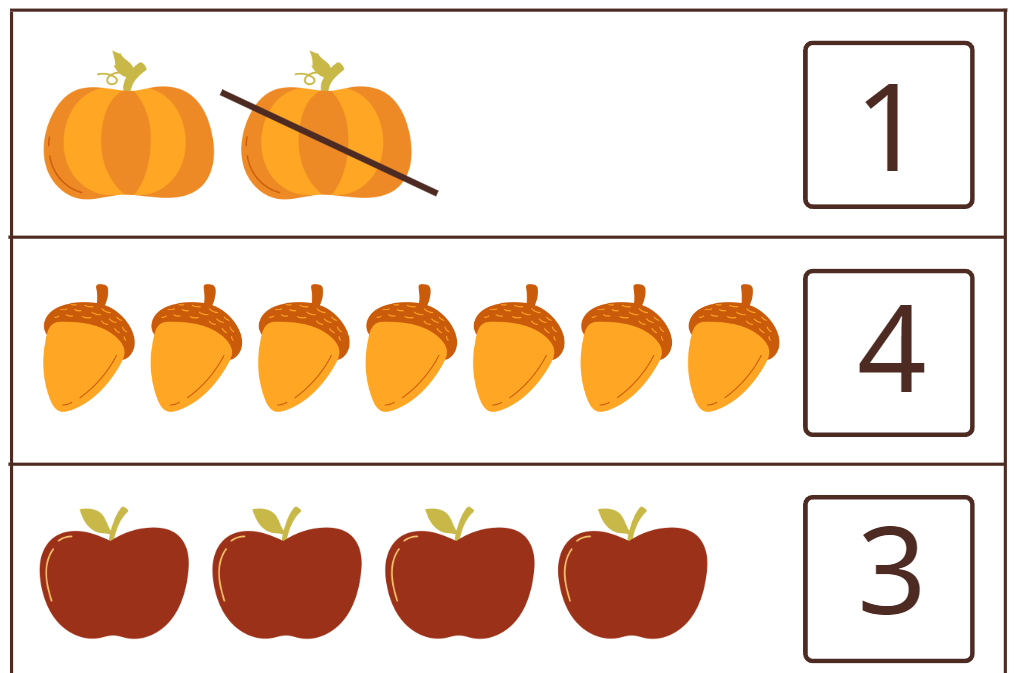
\includegraphics[width=0.32\linewidth]{p14_image1.png}\hfill
        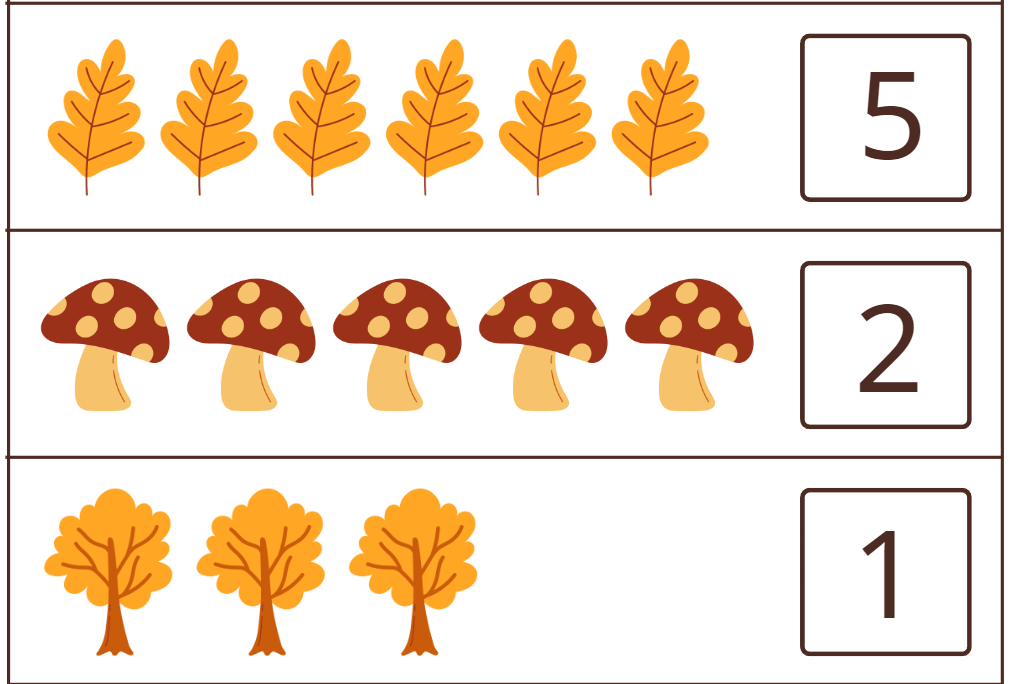
\includegraphics[width=0.32\linewidth]{p14_image2.png}\hfill
        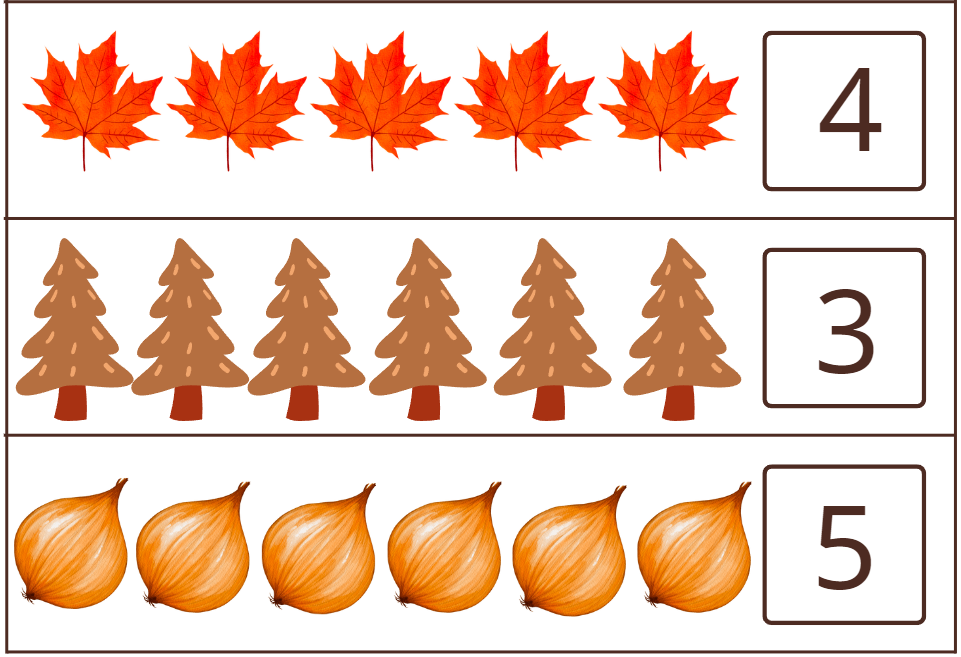
\includegraphics[width=0.32\linewidth]{p14_image3.png}\par}
\end{bt}

\begin{bt}
    Bé hãy gạch bớt để được số lượng con vật còn lại tương ứng với số ở mỗi hình theo mẫu.
    \TThinh[3.4cm]{p14_image4.png}
    \TThinh[3.4cm]{p14_image5.png}
    \TThinh[3.4cm]{p14_image6.png}
    \TThinh[3.4cm]{p14_image7.png}
    \TThinh[3.4cm]{p14_image8.png}
\end{bt}

\begin{bt}
    Bé hãy tô màu đáp án của các phép trừ sau:
    \TThinh[7.5cm]{p14_image9.png}
    \TThinh[7.5cm]{p14_image10.png}
\end{bt}

\begin{bt}
    Bé hãy gạch bớt để thể hiện phép trừ bên dưới và tô màu các con vật còn lại theo mẫu.
    \TThinh[5.2cm]{p14_image11.png}
    \TThinh[5.2cm]{p14_image12.png}
    \TThinh[5.2cm]{p14_image13.png}
\end{bt}

\begin{bt}
    Bé hãy điền số dưa hấu còn lại theo mẫu.
    \TTbatdauhinh
    {\centering
        \fbox{\PKhangtru{\PKduahau}{3}{1}{3 $-$ 1}{\textcolor{PKdo}{\bfseries 2}}}\\[10pt]
        \PKhangtru{\PKduahau}{2}{1}{2 $-$ 1}{}\\[10pt]
        \PKhangtru{\PKduahau}{3}{2}{3 $-$ 2}{}\\[10pt]
        \PKhangtru{\PKduahau}{5}{2}{5 $-$ 2}{}\\[10pt]
        \PKhangtru{\PKduahau}{4}{3}{4 $-$ 3}{}\\[10pt]
        \PKhangtru{\PKduahau}{6}{3}{6 $-$ 3}{}\par}
\end{bt}

\begin{bt}
    Bé tô màu hình sau:
    \TThinh[13cm]{p14_image16.png}
    \TTbatdauhinh
    {\centering
        \begin{minipage}{0.48\linewidth}\centering\PKbutsap{1}{nâu}{PKnau}\\[8pt]\PKbutsap{2}{vàng}{PKvang}\end{minipage}\hfill
        \begin{minipage}{0.48\linewidth}\centering\PKbutsap{3}{trắng}{white}\\[8pt]\PKbutsap{4}{hồng}{PKhong}\end{minipage}\par}
\end{bt}

\begin{bt}
    Bé hãy nối mảnh ghép vào vị trí đúng.
    \TThinh[17cm]{p14_image18.png}
\end{bt}

\begin{bt}
    Bé hãy điền số quả dâu còn lại vào phép tính.
    \TTbatdauhinh
    {\centering
        \PKhangtru{\PKdau}{4}{2}{4 $-$ 2}{}\\[8pt]
        \PKhangtru{\PKdau}{3}{1}{3 $-$ 1}{}\\[8pt]
        \PKhangtru{\PKdau}{5}{3}{5 $-$ 3}{}\\[8pt]
        \PKhangtru{\PKdau}{2}{1}{2 $-$ 1}{}\\[8pt]
        \PKhangtru{\PKdau}{5}{2}{5 $-$ 2}{}\\[8pt]
        \PKhangtru{\PKdau}{3}{3}{3 $-$ 3}{}\par}
\end{bt}

%---------- Bài bổ sung (Toán) ----------
\begin{bt}
    Bé hãy quan sát tranh rồi viết phép trừ thích hợp.
    \TTbatdauhinh
    {\centering
    \begin{tikzpicture}[font=\sffamily\Large]
        % a) 5 quả bóng, 2 quả bay đi
        \node[font=\bfseries] at (-0.4,2.1) {a)};
        \foreach \x/\mau in {0.4/PKdo,1.2/PKxanhla,2.0/PKvang}{
            \begin{scope}[shift={(\x,1.2)}]\PKbong{\mau}\end{scope}
            \draw[gray!70!black] (\x,0.74) .. controls (\x+0.1,0.3) .. (1.2,-0.2);}
        \fill[PKnau] (1.05,-0.35) rectangle (1.35,-0.2);
        \foreach \x/\y/\mau in {4.0/2.3/PKxanhnuoc,4.9/2.6/PKhong}{
            \begin{scope}[shift={(\x,\y)},rotate=-12]\PKbong{\mau}\draw[gray!70!black] (0,-0.46) .. controls (0.15,-0.8) and (-0.1,-1.0) .. (0.05,-1.25);\end{scope}}
        % mũi tên chỉ hướng bóng bay đi (nằm bên trái, không chạm bóng và dây)
        \draw[->,gray,thick,dashed] (2.55,0.55) to[bend left=20] (3.3,1.35);
        \foreach \x in {0,1.7,3.4}{\node[draw,thick,rounded corners=3pt,minimum size=0.9cm] at (\x+0.4,-1.3) {};}
        \node at (1.25,-1.3) {$-$}; \node at (2.95,-1.3) {$=$};
        % b) 4 con cá, 1 con bơi đi
        \begin{scope}[shift={(8.2,0)}]
            \node[font=\bfseries] at (-0.6,2.1) {b)};
            \draw[PKxanhnuoc,thick,fill=PKxanhnuoc!12,rounded corners=12pt] (-0.4,-0.3) rectangle (3.25,2.3);
            \foreach \x/\y/\mau in {0.75/1.55/PKcam,2.3/1.65/PKvang,0.85/0.45/PKhong,2.4/0.5/PKxanhla}{
                \begin{scope}[shift={(\x,\y)},scale=1.1]\PKcadep{\mau}\end{scope}}
            \begin{scope}[shift={(4.65,1.2)},scale=1.1]\PKcadep{PKcam}\end{scope}
            \draw[->,gray,thick,dashed] (3.35,1.05) -- (3.75,1.15);
            \foreach \x in {0,1.7,3.4}{\node[draw,thick,rounded corners=3pt,minimum size=0.9cm] at (\x+0.4,-1.3) {};}
            \node at (1.25,-1.3) {$-$}; \node at (2.95,-1.3) {$=$};
        \end{scope}
    \end{tikzpicture}\par}
\end{bt}

\begin{bt}
    Bé hãy nối mỗi quả táo với ngôi sao ghi kết quả đúng.
    \TTbatdauhinh
    {\centering
    \begin{tikzpicture}
        \foreach \pt/\x in {5 $-$ 1/0,3 $-$ 2/3.2,4 $-$ 2/6.4,5 $-$ 2/9.6,2 $-$ 2/12.8}{
            \begin{scope}[shift={(\x,2.6)},scale=1.25]\PKtao{\pt}\end{scope}
            \fill (\x,1.75) circle (2.5pt);}
        \foreach \so/\x in {2/0,0/3.2,4/6.4,3/9.6,1/12.8}{
            \begin{scope}[shift={(\x,0)}]\PKsao{\so}\end{scope}
            \fill (\x,0.78) circle (2.5pt);}
    \end{tikzpicture}\par}
\end{bt}

\begin{bt}
    Bé giúp bạn bọ rùa điền số thích hợp vào ô trống.
    \TTbatdauhinh
    {\centering
    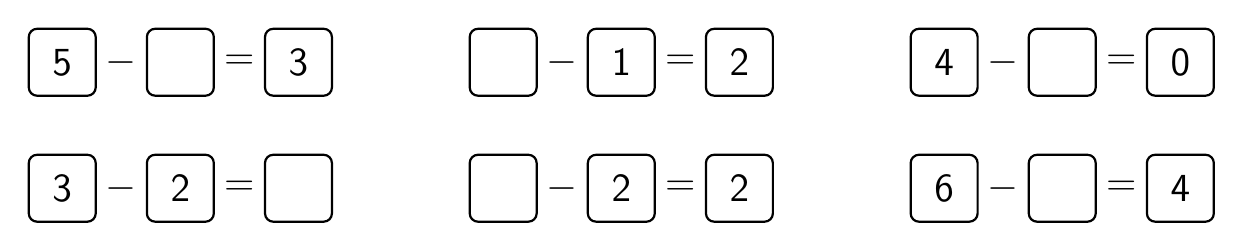
\begin{tikzpicture}[font=\sffamily\Large]
        \foreach \a/\b/\c [count=\k] in {5/{}/3,{}/1/2,4/{}/0,3/2/{},{}/2/2,6/{}/4}{
            \pgfmathtruncatemacro{\cot}{mod(\k-1,3)}\pgfmathtruncatemacro{\hang}{div(\k-1,3)}
            \begin{scope}[shift={(5.6*\cot,-1.6*\hang)}]
                \begin{scope}[shift={(-0.2,0)},scale=1.1]\PKborua\end{scope}
                \node[draw,thick,rounded corners=3pt,minimum size=0.85cm] at (0.9,0) {\a};
                \node at (1.65,0) {$-$};
                \node[draw,thick,rounded corners=3pt,minimum size=0.85cm] at (2.4,0) {\b};
                \node at (3.15,0) {$=$};
                \node[draw,thick,rounded corners=3pt,minimum size=0.85cm] at (3.9,0) {\c};
            \end{scope}}
    \end{tikzpicture}\par}
\end{bt}

%%%%%%%%%%%%%%%%%%%%%%%%%%%%%%%%%%%%%%%%%%%%%%%%%%%%%%%%%%
%                  PHIẾU TIẾNG VIỆT
%%%%%%%%%%%%%%%%%%%%%%%%%%%%%%%%%%%%%%%%%%%%%%%%%%%%%%%%%%
\newpage
\TTdatlaibai
{\centering
        {\color{mauchinh!120}\bfseries\Large PHIẾU BÀI TẬP TIẾNG VIỆT PRE1 -- TUẦN 14}\\[3pt]
        {\color{mauchinh!120}\bfseries\Large CHỦ ĐỀ 14: LÀM QUEN ÂM D, Đ}\par}
\vspace{6pt}
\TTthongtin

\begin{bt}
    Bé hãy đọc và khoanh vào âm \textbf{d} của các từ phía dưới.
    \TThinh[2.6cm]{p14_image20.png}
    \TTbatdauhinh
    {\centering
        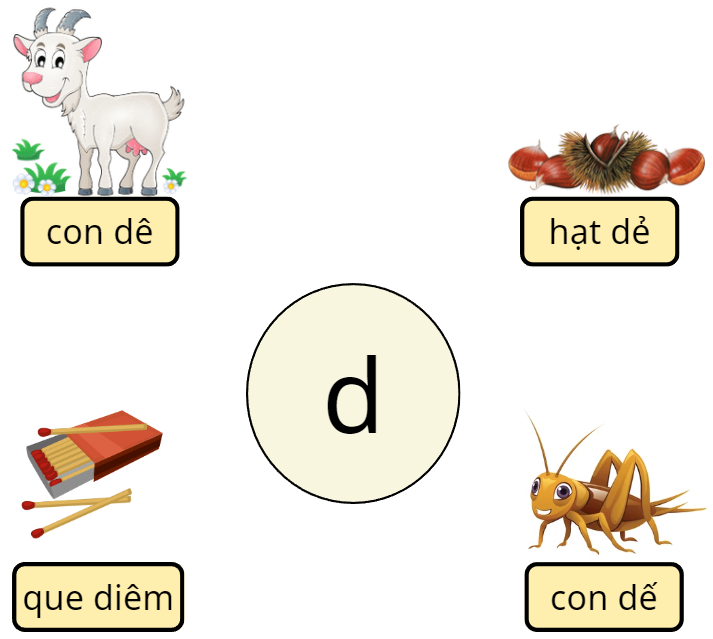
\includegraphics[height=6.2cm]{p14_image21.png}\hfill
        \begin{minipage}[b]{0.42\linewidth}\centering\PKghep{d}{ê}{dê}\\[8pt]\PKghep{d}{ế}{dế}\end{minipage}\par}
\end{bt}

\begin{bt}
    Bé hãy đọc và khoanh vào âm \textbf{đ} của các từ phía dưới.
    \TThinh[2.6cm]{p14_image23.png}
    \TTbatdauhinh
    {\centering
        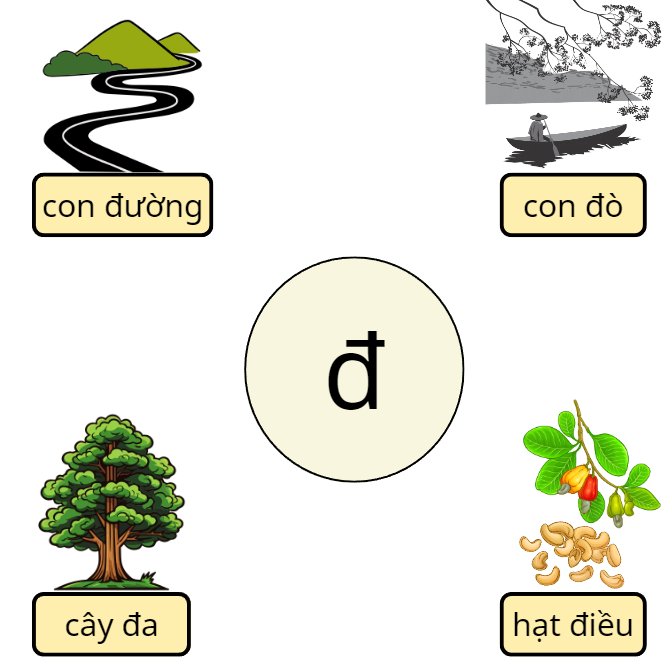
\includegraphics[height=6.2cm]{p14_image24.png}\hfill
        \begin{minipage}[b]{0.42\linewidth}\centering\PKghep{đ}{o}{đo}\\[8pt]\PKghep{đ}{ò}{đò}\end{minipage}\par}
\end{bt}

\begin{bt}
    Bé hãy tô màu \textbf{xanh dương} vào giọt nước có từ chứa chữ \textbf{d} và tô màu \textbf{hồng} vào giọt nước có từ chứa chữ \textbf{đ}.
    \TTbatdauhinh
    {\centering
    \begin{tikzpicture}[scale=1.15]
        \foreach \tu/\x/\y in {đi/0/0.2,dừa/1.9/-0.1,đua/3.8/0.15,dế/5.7/-0.15,đỏ/7.6/0.2,
                               dê/0.9/-2.3,đói/2.8/-2.0,đậu/4.7/-2.35,đi/6.6/-2.05,diều/8.5/-2.3}{
            \begin{scope}[shift={(\x,\y)}]\PKgiot{\tu}\end{scope}}
    \end{tikzpicture}\par}
\end{bt}

\begin{bt}
    Bé hãy nối tên với hình ảnh tương ứng.
    \TThinh[8cm]{p14_image27.png}
\end{bt}

\begin{bt}
    Bé hãy viết và đọc các từ sau:
    \TThinh[10cm]{p14_image28.png}
\end{bt}

\begin{bt}
    Nối tên các con vật với dấu phù hợp.
    \TThinh[10cm]{p14_image29.png}
\end{bt}

\begin{bt}
    Bé hãy viết chữ \textbf{d}.
    \TThinh[5.5cm]{p14_image30.png}
    \TThinh[3.6cm]{p14_image31.png}
    \TThinh[5.5cm]{p14_image30.png}
    \TThinh[3.6cm]{p14_image31.png}
\end{bt}

\begin{bt}
    Bé hãy viết chữ \textbf{đ}.
    \TThinh[5.5cm]{p14_image32.png}
    \TThinh[3.6cm]{p14_image33.png}
    \TThinh[5.5cm]{p14_image32.png}
    \TThinh[3.6cm]{p14_image33.png}
\end{bt}

%---------- Bài bổ sung (Tiếng Việt) ----------
\begin{bt}
    Bé hãy điền \textbf{d} hay \textbf{đ} vào chỗ chấm.
    \TTbatdauhinh
    {\centering
        \PKoditen{\PKdua}{quả \underline{\hspace{0.7cm}}ừa}\hfill
        \PKoditen{\PKdia}{cái \underline{\hspace{0.7cm}}ĩa}\hfill
        \PKoditen{\PKdo}{con \underline{\hspace{0.7cm}}ò}\\[10pt]
        \PKoditen{\PKdu}{cái \underline{\hspace{0.7cm}}ù}\hfill
        \PKoditen{\PKden}{bóng \underline{\hspace{0.7cm}}èn}\hfill
        \PKoditen{\PKco}{cờ \underline{\hspace{0.7cm}}ỏ}\par}
\end{bt}

\begin{bt}
    Bé hãy tô màu \textbf{xanh} những chú cá mang chữ \textbf{d} và tô màu \textbf{đỏ} những chú cá mang chữ \textbf{đ}.
    \TTbatdauhinh
    {\centering
    \begin{tikzpicture}
        \draw[PKxanhnuoc,very thick,fill=PKxanhnuoc!10,rounded corners=20pt] (-1.2,-3.6) rectangle (14.6,1.2);
        \foreach \x/\y in {1.5/-3.3,5.2/-3.35,9.5/-3.3,13.2/-3.35}{\draw[green!50!black,thick] (\x,\y) .. controls (\x-0.2,\y+0.5) and (\x+0.2,\y+0.8) .. (\x,\y+1.2);}
        \foreach \chu/\x/\y [count=\k] in {d/0.2/0,đ/2.4/0.15,b/4.6/-0.05,d/6.8/0.1,đ/9.0/0,o/11.2/0.12,đ/13.3/-0.05,
                                           đ/1.2/-2.1,d/3.4/-1.95,a/5.6/-2.1,đ/7.8/-1.95,d/10.0/-2.1,d/12.2/-1.95}{
            \begin{scope}[shift={(\x,\y)},scale=1.9]\PKca{white}\end{scope}
            \node[font=\sffamily\bfseries\LARGE] at (\x-0.3,\y) {\chu};}
    \end{tikzpicture}\par}
\end{bt}

\begin{center}
       \faGg\faGg\quad Hết \quad\faGg\faGg
\end{center}
\end{document}
